\documentclass[aspectratio=169]{beamer}

% Default packages
\usepackage[T1]{fontenc}
\usepackage[english]{babel}
\usepackage{pgfplots}
\pgfplotsset{compat=newest}
\usepackage{booktabs}
\usepackage{siunitx}
\usepackage{amsmath}

% Font selection
% Latin Modern
\usepackage{lmodern}
% Verdana font type
%\usepackage{verdana}
% Helvetica
%\usepackage{helvet}
% Times (text and math)
%\usepackage{newtx, newtxmath}
% Nice font combination
%\usepackage{mathptmx} % math
%\usepackage{sourcesanspro} % sans-serif
\usepackage{charter} % serif

%Avoid shaded in RMarkdown
\usepackage{color}
\usepackage{fancyvrb}
\newcommand{\VerbBar}{|}
\newcommand{\VERB}{\Verb[commandchars=\\\{\}]}
\DefineVerbatimEnvironment{Highlighting}{Verbatim}{commandchars=\\\{\}}
% Add ',fontsize=\small' for more characters per line
\usepackage{framed}
\definecolor{shadecolor}{RGB}{248,248,248}
\newenvironment{Shaded}{\begin{snugshade}}{\end{snugshade}}
\newcommand{\AlertTok}[1]{\textcolor[rgb]{0.94,0.16,0.16}{#1}}
\newcommand{\AnnotationTok}[1]{\textcolor[rgb]{0.56,0.35,0.01}{\textbf{\textit{#1}}}}
\newcommand{\AttributeTok}[1]{\textcolor[rgb]{0.77,0.63,0.00}{#1}}
\newcommand{\BaseNTok}[1]{\textcolor[rgb]{0.00,0.00,0.81}{#1}}
\newcommand{\BuiltInTok}[1]{#1}
\newcommand{\CharTok}[1]{\textcolor[rgb]{0.31,0.60,0.02}{#1}}
\newcommand{\CommentTok}[1]{\textcolor[rgb]{0.56,0.35,0.01}{\textit{#1}}}
\newcommand{\CommentVarTok}[1]{\textcolor[rgb]{0.56,0.35,0.01}{\textbf{\textit{#1}}}}
\newcommand{\ConstantTok}[1]{\textcolor[rgb]{0.00,0.00,0.00}{#1}}
\newcommand{\ControlFlowTok}[1]{\textcolor[rgb]{0.13,0.29,0.53}{\textbf{#1}}}
\newcommand{\DataTypeTok}[1]{\textcolor[rgb]{0.13,0.29,0.53}{#1}}
\newcommand{\DecValTok}[1]{\textcolor[rgb]{0.00,0.00,0.81}{#1}}
\newcommand{\DocumentationTok}[1]{\textcolor[rgb]{0.56,0.35,0.01}{\textbf{\textit{#1}}}}
\newcommand{\ErrorTok}[1]{\textcolor[rgb]{0.64,0.00,0.00}{\textbf{#1}}}
\newcommand{\ExtensionTok}[1]{#1}
\newcommand{\FloatTok}[1]{\textcolor[rgb]{0.00,0.00,0.81}{#1}}
\newcommand{\FunctionTok}[1]{\textcolor[rgb]{0.00,0.00,0.00}{#1}}
\newcommand{\ImportTok}[1]{#1}
\newcommand{\InformationTok}[1]{\textcolor[rgb]{0.56,0.35,0.01}{\textbf{\textit{#1}}}}
\newcommand{\KeywordTok}[1]{\textcolor[rgb]{0.13,0.29,0.53}{\textbf{#1}}}
\newcommand{\NormalTok}[1]{#1}
\newcommand{\OperatorTok}[1]{\textcolor[rgb]{0.81,0.36,0.00}{\textbf{#1}}}
\newcommand{\OtherTok}[1]{\textcolor[rgb]{0.56,0.35,0.01}{#1}}
\newcommand{\PreprocessorTok}[1]{\textcolor[rgb]{0.56,0.35,0.01}{\textit{#1}}}
\newcommand{\RegionMarkerTok}[1]{#1}
\newcommand{\SpecialCharTok}[1]{\textcolor[rgb]{0.00,0.00,0.00}{#1}}
\newcommand{\SpecialStringTok}[1]{\textcolor[rgb]{0.31,0.60,0.02}{#1}}
\newcommand{\StringTok}[1]{\textcolor[rgb]{0.31,0.60,0.02}{#1}}
\newcommand{\VariableTok}[1]{\textcolor[rgb]{0.00,0.00,0.00}{#1}}
\newcommand{\VerbatimStringTok}[1]{\textcolor[rgb]{0.31,0.60,0.02}{#1}}
\newcommand{\WarningTok}[1]{\textcolor[rgb]{0.56,0.35,0.01}{\textbf{\textit{#1}}}}



% Use DTU theme, see below for options
\usetheme[department=compute]{DTU}

\title[Automated and Early Detection of Disease Outbreaks]{Farrington
and Noufaily}
\author{Kasper Schou Telkamp}
\institute{Section for Dynamical Systems}
\date{2023-03-02}
	
\newcommand{\tabitem}{{\color{dtured}$\bullet$} }

\DeclareMathOperator{\E}{E}
\DeclareMathOperator{\G}{G}
\DeclareMathOperator{\N}{N}
\DeclareMathOperator{\NB}{NB}
\DeclareMathOperator{\Pois}{Pois}
\DeclareMathOperator{\Geom}{Geom}


\begin{document}


\frame{
	\maketitle
}

\frame{
	\frametitle{Outline}
	\tableofcontents
}

\hypertarget{data-exploration}{%
\section{Data exploration}\label{data-exploration}}

\hypertarget{vtec-stec}{%
\subsection*{VTEC / STEC}\label{vtec-stec}}

\begin{frame}{VTEC / STEC}
\tiny

\begin{table}
\centering\begingroup\fontsize{12}{14}\selectfont

\begin{tabular}{llll}
\toprule
Date & ageGroup & y & n\\
\midrule
2008-01-01 & <1 year & 2 & 64137\\
2008-01-01 & 1-4 years & 2 & 259910\\
2008-01-01 & 5-14 years & 2 & 680529\\
2008-01-01 & 15-24 years & 1 & 631724\\
... & ... & ... & ...\\
2022-12-01 & 55-64 years & 2 & 773073\\
2022-12-01 & 65-74 years & 5 & 621965\\
2022-12-01 & 75-84 years & 4 & 449423\\
2022-12-01 & 85+ years & 3 & 132181\\
\bottomrule
\end{tabular}
\endgroup{}
\end{table}

\normalsize
\end{frame}

\hypertarget{vtec-stec-1}{%
\subsection{VTEC / STEC}\label{vtec-stec-1}}

\begin{frame}{VTEC / STEC}
\tiny

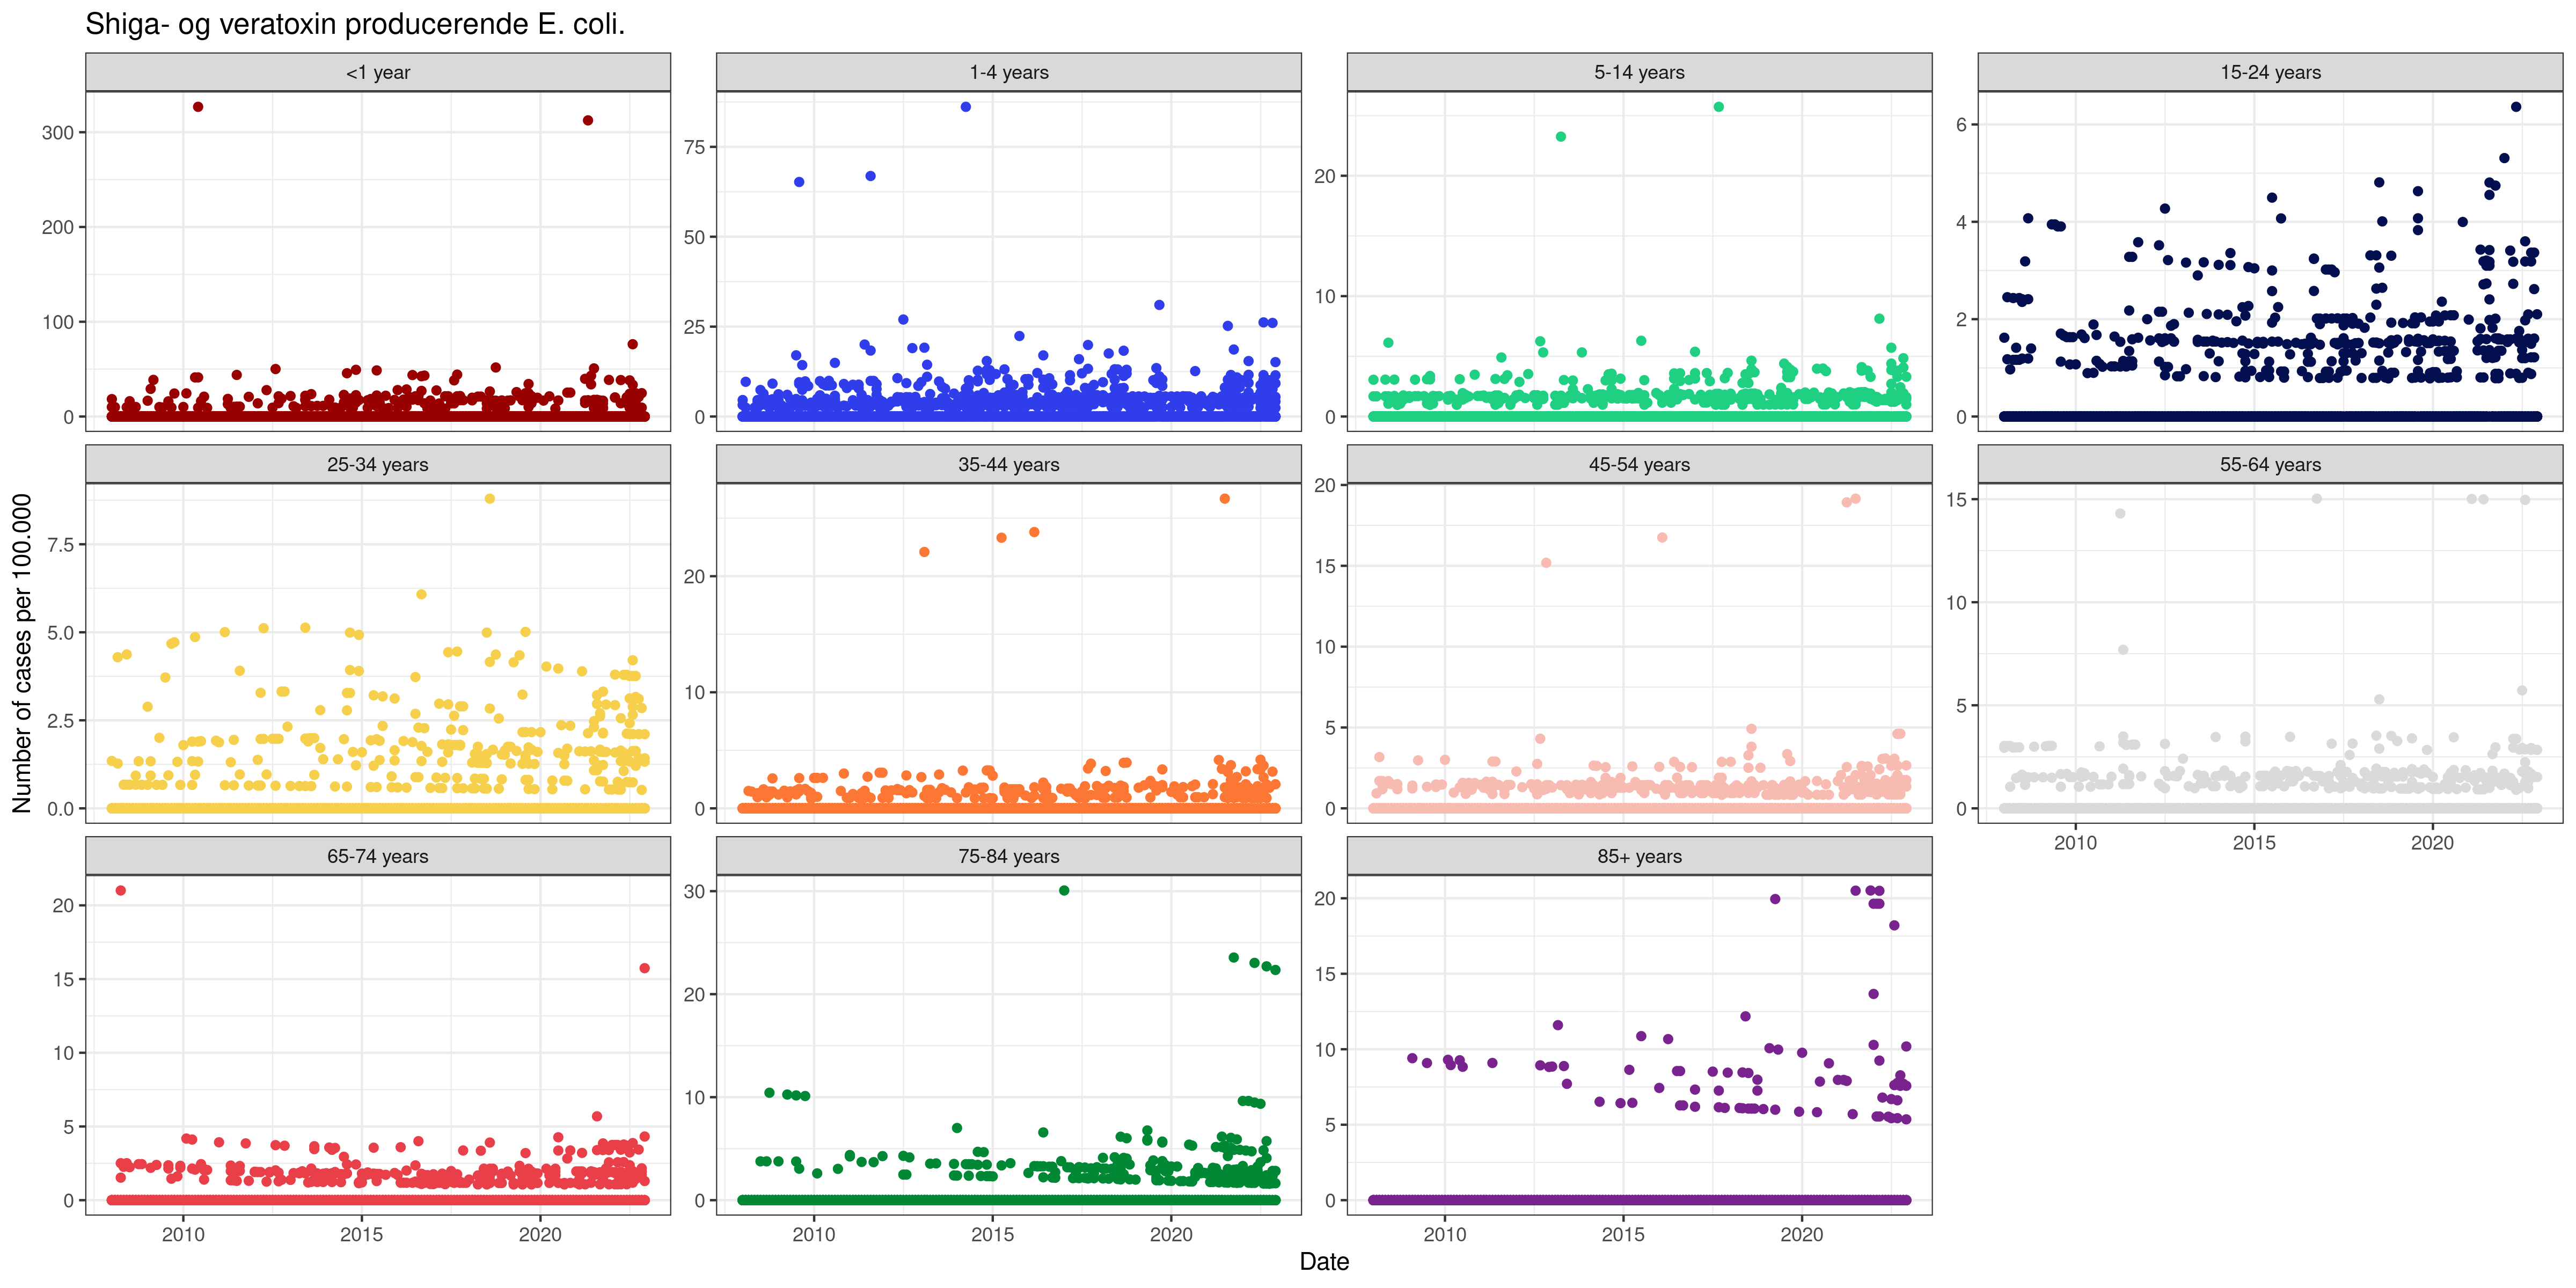
\includegraphics[width=1\linewidth]{../figures/ShigaogveratoxinproducerendeEcolixAgeGroup}

\normalsize
\end{frame}

\hypertarget{prepare-the-data-for-modelling-with-surveillance}{%
\subsection{\texorpdfstring{Prepare the data for modelling with
\texttt{surveillance}}{Prepare the data for modelling with surveillance}}\label{prepare-the-data-for-modelling-with-surveillance}}

\begin{frame}[fragile]{Prepare the data for modelling with
\texttt{surveillance}}
\tiny

\begin{Shaded}
\begin{Highlighting}[]
\CommentTok{\# Import libraries}
\FunctionTok{library}\NormalTok{(readr)}
\FunctionTok{library}\NormalTok{(dplyr)}
\FunctionTok{library}\NormalTok{(tidyr)}
\FunctionTok{library}\NormalTok{(surveillance)}

\CommentTok{\# Import the data}
\NormalTok{dat }\OtherTok{\textless{}{-}} \FunctionTok{read\_rds}\NormalTok{(}\AttributeTok{file =} \StringTok{"../../data/processed/dat.rds"}\NormalTok{)}

\CommentTok{\# Only consider some of the data}
\NormalTok{y }\OtherTok{\textless{}{-}}\NormalTok{ dat }\SpecialCharTok{\%\textgreater{}\%}
  \FunctionTok{filter}\NormalTok{(caseDef }\SpecialCharTok{==} \StringTok{"Shiga{-} og veratoxin producerende E. coli."}\NormalTok{) }\SpecialCharTok{\%\textgreater{}\%}
  \FunctionTok{group\_by}\NormalTok{(Date, ageGroup) }\SpecialCharTok{\%\textgreater{}\%}
  \FunctionTok{reframe}\NormalTok{(}\AttributeTok{y =} \FunctionTok{sum}\NormalTok{(cases), }\AttributeTok{n =} \FunctionTok{sum}\NormalTok{(n))}

\CommentTok{\# Widen observations into a matrix format}
\NormalTok{observed }\OtherTok{\textless{}{-}}\NormalTok{ y }\SpecialCharTok{\%\textgreater{}\%}
  \FunctionTok{select}\NormalTok{(}\SpecialCharTok{{-}}\NormalTok{n) }\SpecialCharTok{\%\textgreater{}\%}
  \FunctionTok{pivot\_wider}\NormalTok{(}
    \AttributeTok{names\_from =} \FunctionTok{c}\NormalTok{(ageGroup),}
    \AttributeTok{names\_sep =} \StringTok{"."}\NormalTok{,}
    \AttributeTok{values\_from =}\NormalTok{ y) }\SpecialCharTok{\%\textgreater{}\%}
  \FunctionTok{arrange}\NormalTok{(Date)}

\CommentTok{\# Widen population sizes into a matrix format}
\NormalTok{population }\OtherTok{\textless{}{-}}\NormalTok{ y }\SpecialCharTok{\%\textgreater{}\%}
  \FunctionTok{select}\NormalTok{(}\SpecialCharTok{{-}}\NormalTok{y) }\SpecialCharTok{\%\textgreater{}\%}
  \FunctionTok{pivot\_wider}\NormalTok{(}
    \AttributeTok{names\_from =} \FunctionTok{c}\NormalTok{(ageGroup),}
    \AttributeTok{names\_sep =} \StringTok{"."}\NormalTok{,}
    \AttributeTok{values\_from =}\NormalTok{ n) }\SpecialCharTok{\%\textgreater{}\%}
  \FunctionTok{arrange}\NormalTok{(Date)}

\CommentTok{\# Convert observations into an \textquotesingle{}sts\textquotesingle{} class}
\NormalTok{STEC }\OtherTok{\textless{}{-}} \FunctionTok{sts}\NormalTok{(}
  \AttributeTok{observed =}\NormalTok{ observed[,}\SpecialCharTok{{-}}\DecValTok{1}\NormalTok{],}
  \AttributeTok{epoch =}\NormalTok{ observed}\SpecialCharTok{$}\NormalTok{Date,}
  \AttributeTok{epochAsDate =} \ConstantTok{TRUE}\NormalTok{,}
  \AttributeTok{frequency =} \DecValTok{12}\NormalTok{,}
  \AttributeTok{population =} \FunctionTok{as.matrix}\NormalTok{(population[,}\SpecialCharTok{{-}}\DecValTok{1}\NormalTok{])}
\NormalTok{  )}
\end{Highlighting}
\end{Shaded}

\normalsize
\end{frame}

\hypertarget{farrington}{%
\section{Farrington}\label{farrington}}

\hypertarget{implementation}{%
\subsection{Implementation}\label{implementation}}

\begin{frame}[fragile]{Implementation}
\tiny

\begin{Shaded}
\begin{Highlighting}[]
\CommentTok{\# Specify the controls for the Farrington method}
\NormalTok{con.farrington }\OtherTok{\textless{}{-}} \FunctionTok{list}\NormalTok{(}
  \AttributeTok{range =} \ConstantTok{NULL}\NormalTok{, }\AttributeTok{b =} \DecValTok{5}\NormalTok{, }\AttributeTok{w =} \DecValTok{3}\NormalTok{,}
  \AttributeTok{reweight =} \ConstantTok{TRUE}\NormalTok{, }\AttributeTok{weightsThreshold =} \DecValTok{1}\NormalTok{,}
  \AttributeTok{verbose =} \ConstantTok{TRUE}\NormalTok{, }\AttributeTok{glmWarnings =} \ConstantTok{TRUE}\NormalTok{,}
  \AttributeTok{alpha =} \FloatTok{0.05}\NormalTok{, }\AttributeTok{trend =} \ConstantTok{TRUE}\NormalTok{, }\AttributeTok{pThresholdTrend =} \FloatTok{0.05}\NormalTok{,}
  \AttributeTok{limit54 =} \FunctionTok{c}\NormalTok{(}\DecValTok{5}\NormalTok{,}\DecValTok{4}\NormalTok{), }\AttributeTok{powertrans =} \StringTok{"2/3"}\NormalTok{,}
  \AttributeTok{fitFun =} \StringTok{"algo.farrington.fitGLM.flexible"}\NormalTok{,}
  \AttributeTok{populationOffset =} \ConstantTok{TRUE}\NormalTok{,}
  \AttributeTok{noPeriods =} \DecValTok{1}\NormalTok{, }\AttributeTok{pastWooksNotIncluded =} \ConstantTok{NULL}\NormalTok{,}
  \AttributeTok{thersholdMethod =} \StringTok{"delta"}
\NormalTok{)}

\CommentTok{\# Execute the Farrington method}
\NormalTok{STEC\_farrington }\OtherTok{\textless{}{-}} \FunctionTok{farringtonFlexible}\NormalTok{(}\AttributeTok{sts =}\NormalTok{ STEC, con.farrington)}
\end{Highlighting}
\end{Shaded}

\normalsize
\end{frame}

\hypertarget{results}{%
\subsection{Results}\label{results}}

\begin{frame}{Results}
\tiny

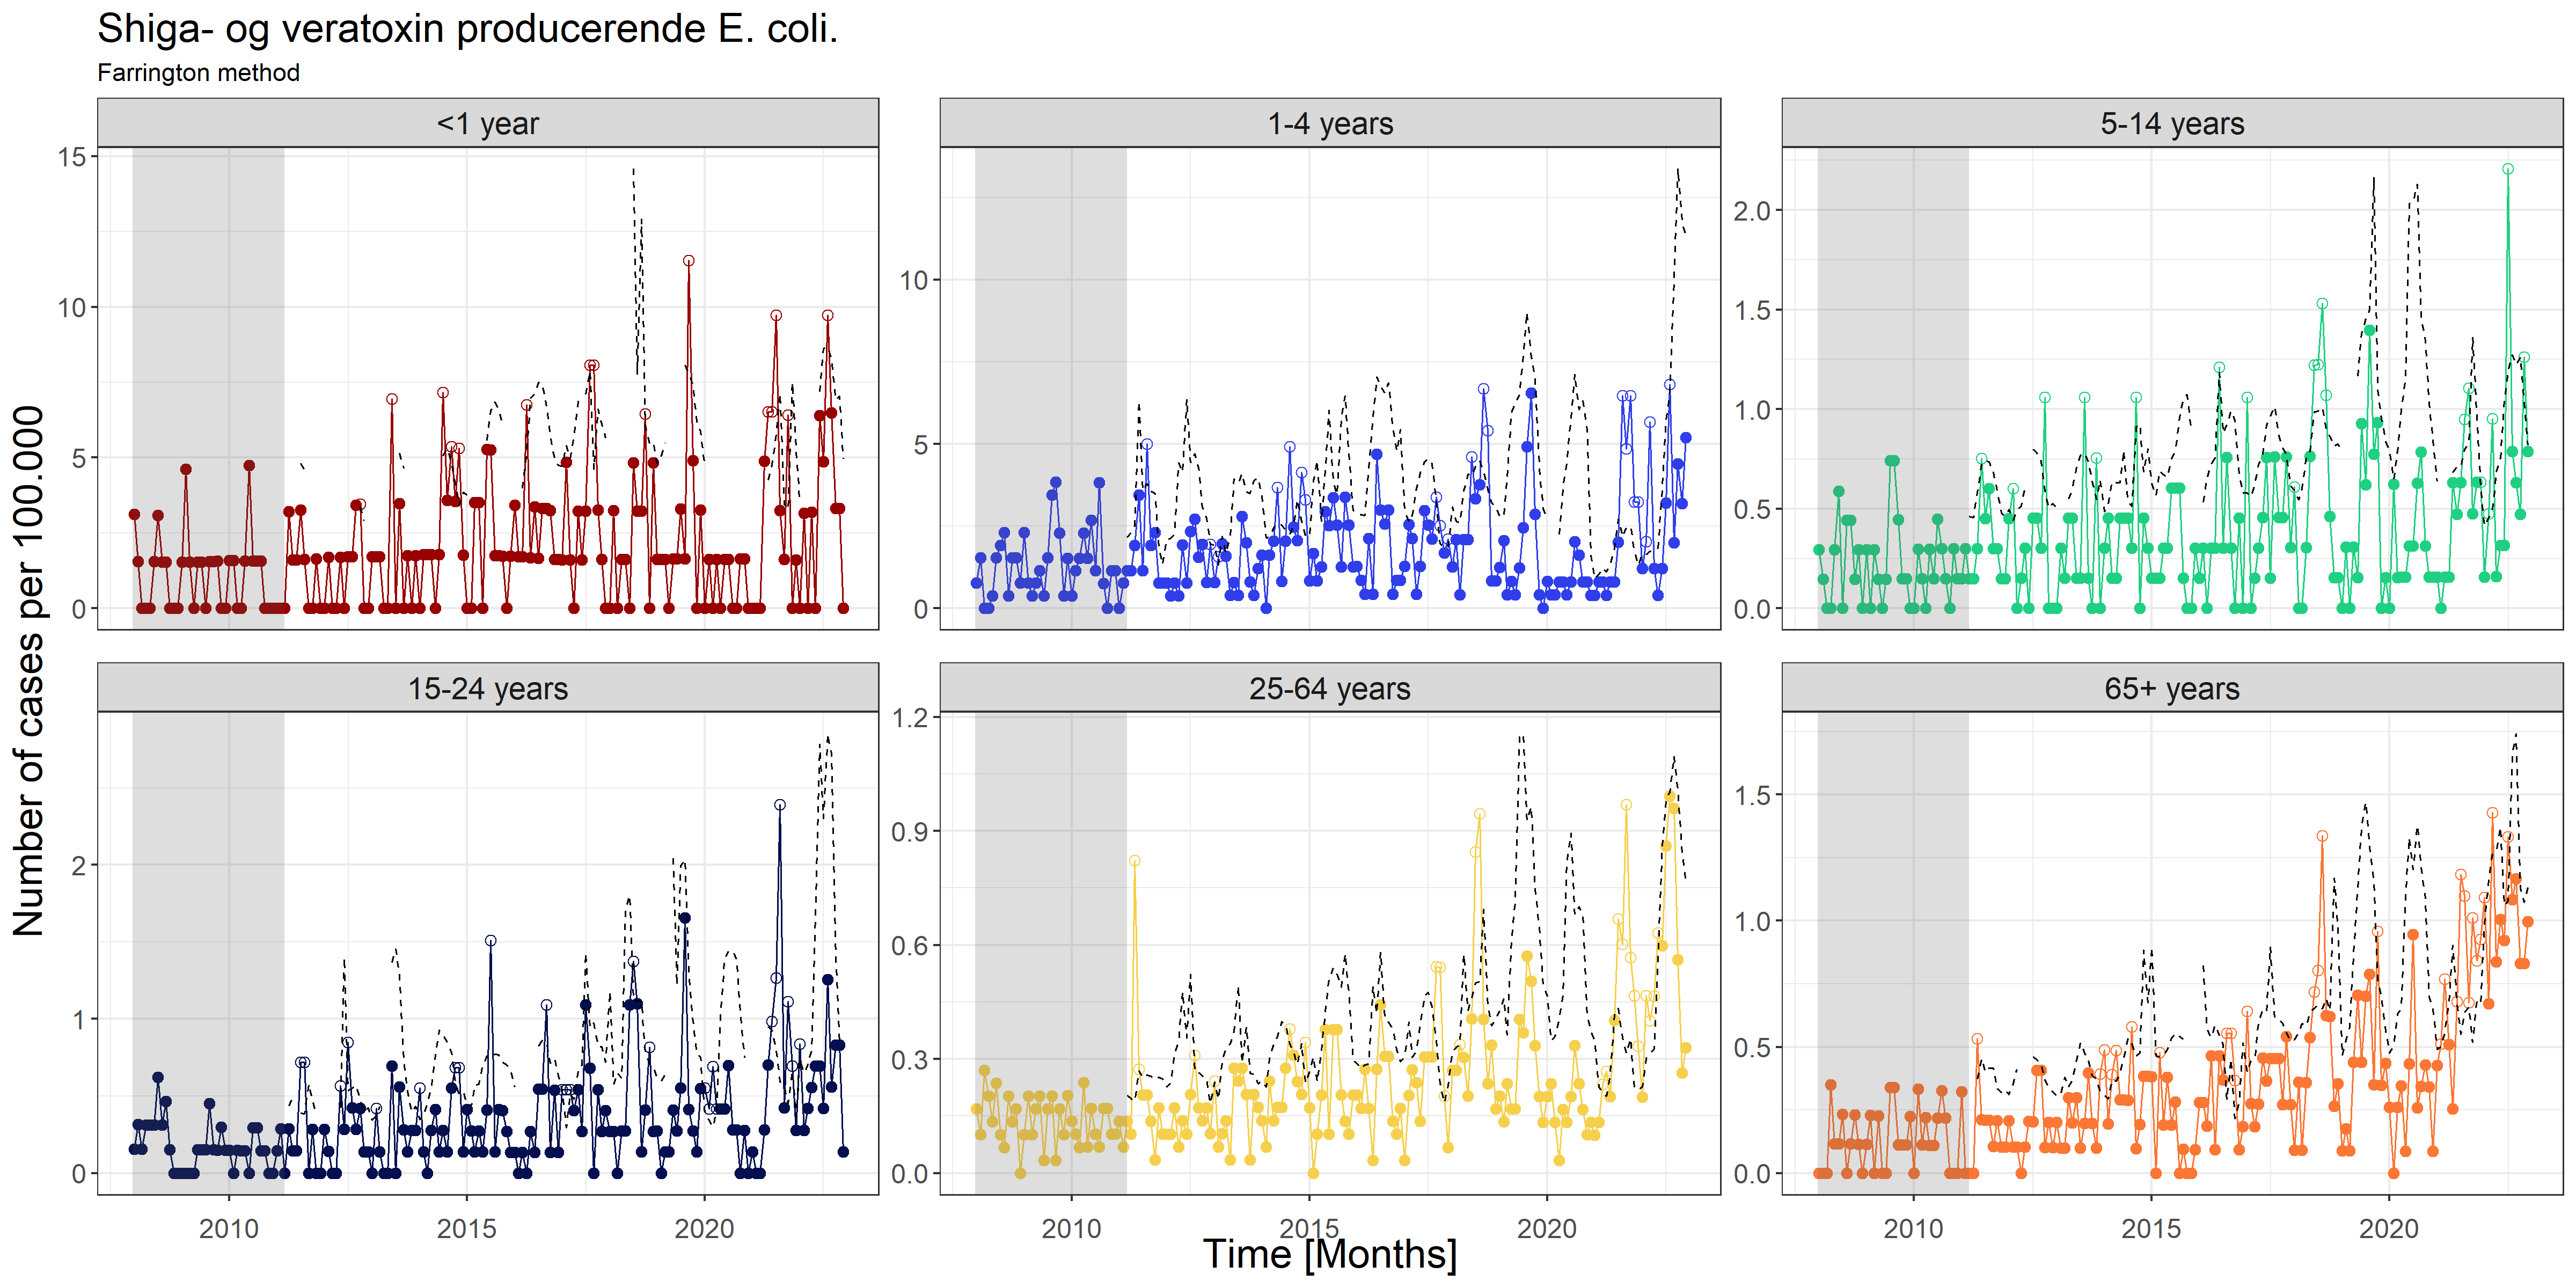
\includegraphics[width=1\linewidth]{../figures/STEC_farrington}

\normalsize
\end{frame}

\hypertarget{noufaily}{%
\section{Noufaily}\label{noufaily}}

\hypertarget{implementation-1}{%
\subsection{Implementation}\label{implementation-1}}

\begin{frame}[fragile]{Implementation}
\tiny

\begin{Shaded}
\begin{Highlighting}[]
\CommentTok{\# Specify the controls for the Noufaily method}
\NormalTok{con.noufaily }\OtherTok{\textless{}{-}} \FunctionTok{list}\NormalTok{(}
  \AttributeTok{range =} \ConstantTok{NULL}\NormalTok{, }\AttributeTok{b =} \DecValTok{5}\NormalTok{, }\AttributeTok{w =} \DecValTok{3}\NormalTok{,}
  \AttributeTok{reweight =} \ConstantTok{TRUE}\NormalTok{, }\AttributeTok{weightsThreshold =} \FloatTok{2.58}\NormalTok{,}
  \AttributeTok{verbose =} \ConstantTok{TRUE}\NormalTok{, }\AttributeTok{glmWarnings =} \ConstantTok{TRUE}\NormalTok{,}
  \AttributeTok{alpha =} \FloatTok{0.05}\NormalTok{, }\AttributeTok{trend =} \ConstantTok{TRUE}\NormalTok{, }\AttributeTok{pThresholdTrend =} \FloatTok{0.05}\NormalTok{,}
  \AttributeTok{limit54 =} \FunctionTok{c}\NormalTok{(}\DecValTok{5}\NormalTok{,}\DecValTok{4}\NormalTok{), }\AttributeTok{powertrans =} \StringTok{"2/3"}\NormalTok{,}
  \AttributeTok{fitFun =} \StringTok{"algo.farrington.fitGLM.flexible"}\NormalTok{,}
  \AttributeTok{populationOffset =} \ConstantTok{TRUE}\NormalTok{,}
  \AttributeTok{noPeriods =} \DecValTok{1}\NormalTok{, }\AttributeTok{pastWooksNotIncluded =} \ConstantTok{NULL}\NormalTok{,}
  \AttributeTok{thersholdMethod =} \StringTok{"delta"}
\NormalTok{)}

\CommentTok{\# Execute the Noufaily method}
\NormalTok{STEC\_noufaily }\OtherTok{\textless{}{-}} \FunctionTok{farringtonFlexible}\NormalTok{(}\AttributeTok{sts =}\NormalTok{ STEC, con.noufaily)}
\end{Highlighting}
\end{Shaded}

\normalsize
\end{frame}

\hypertarget{results-1}{%
\subsection{Results}\label{results-1}}

\begin{frame}{Results}
\tiny

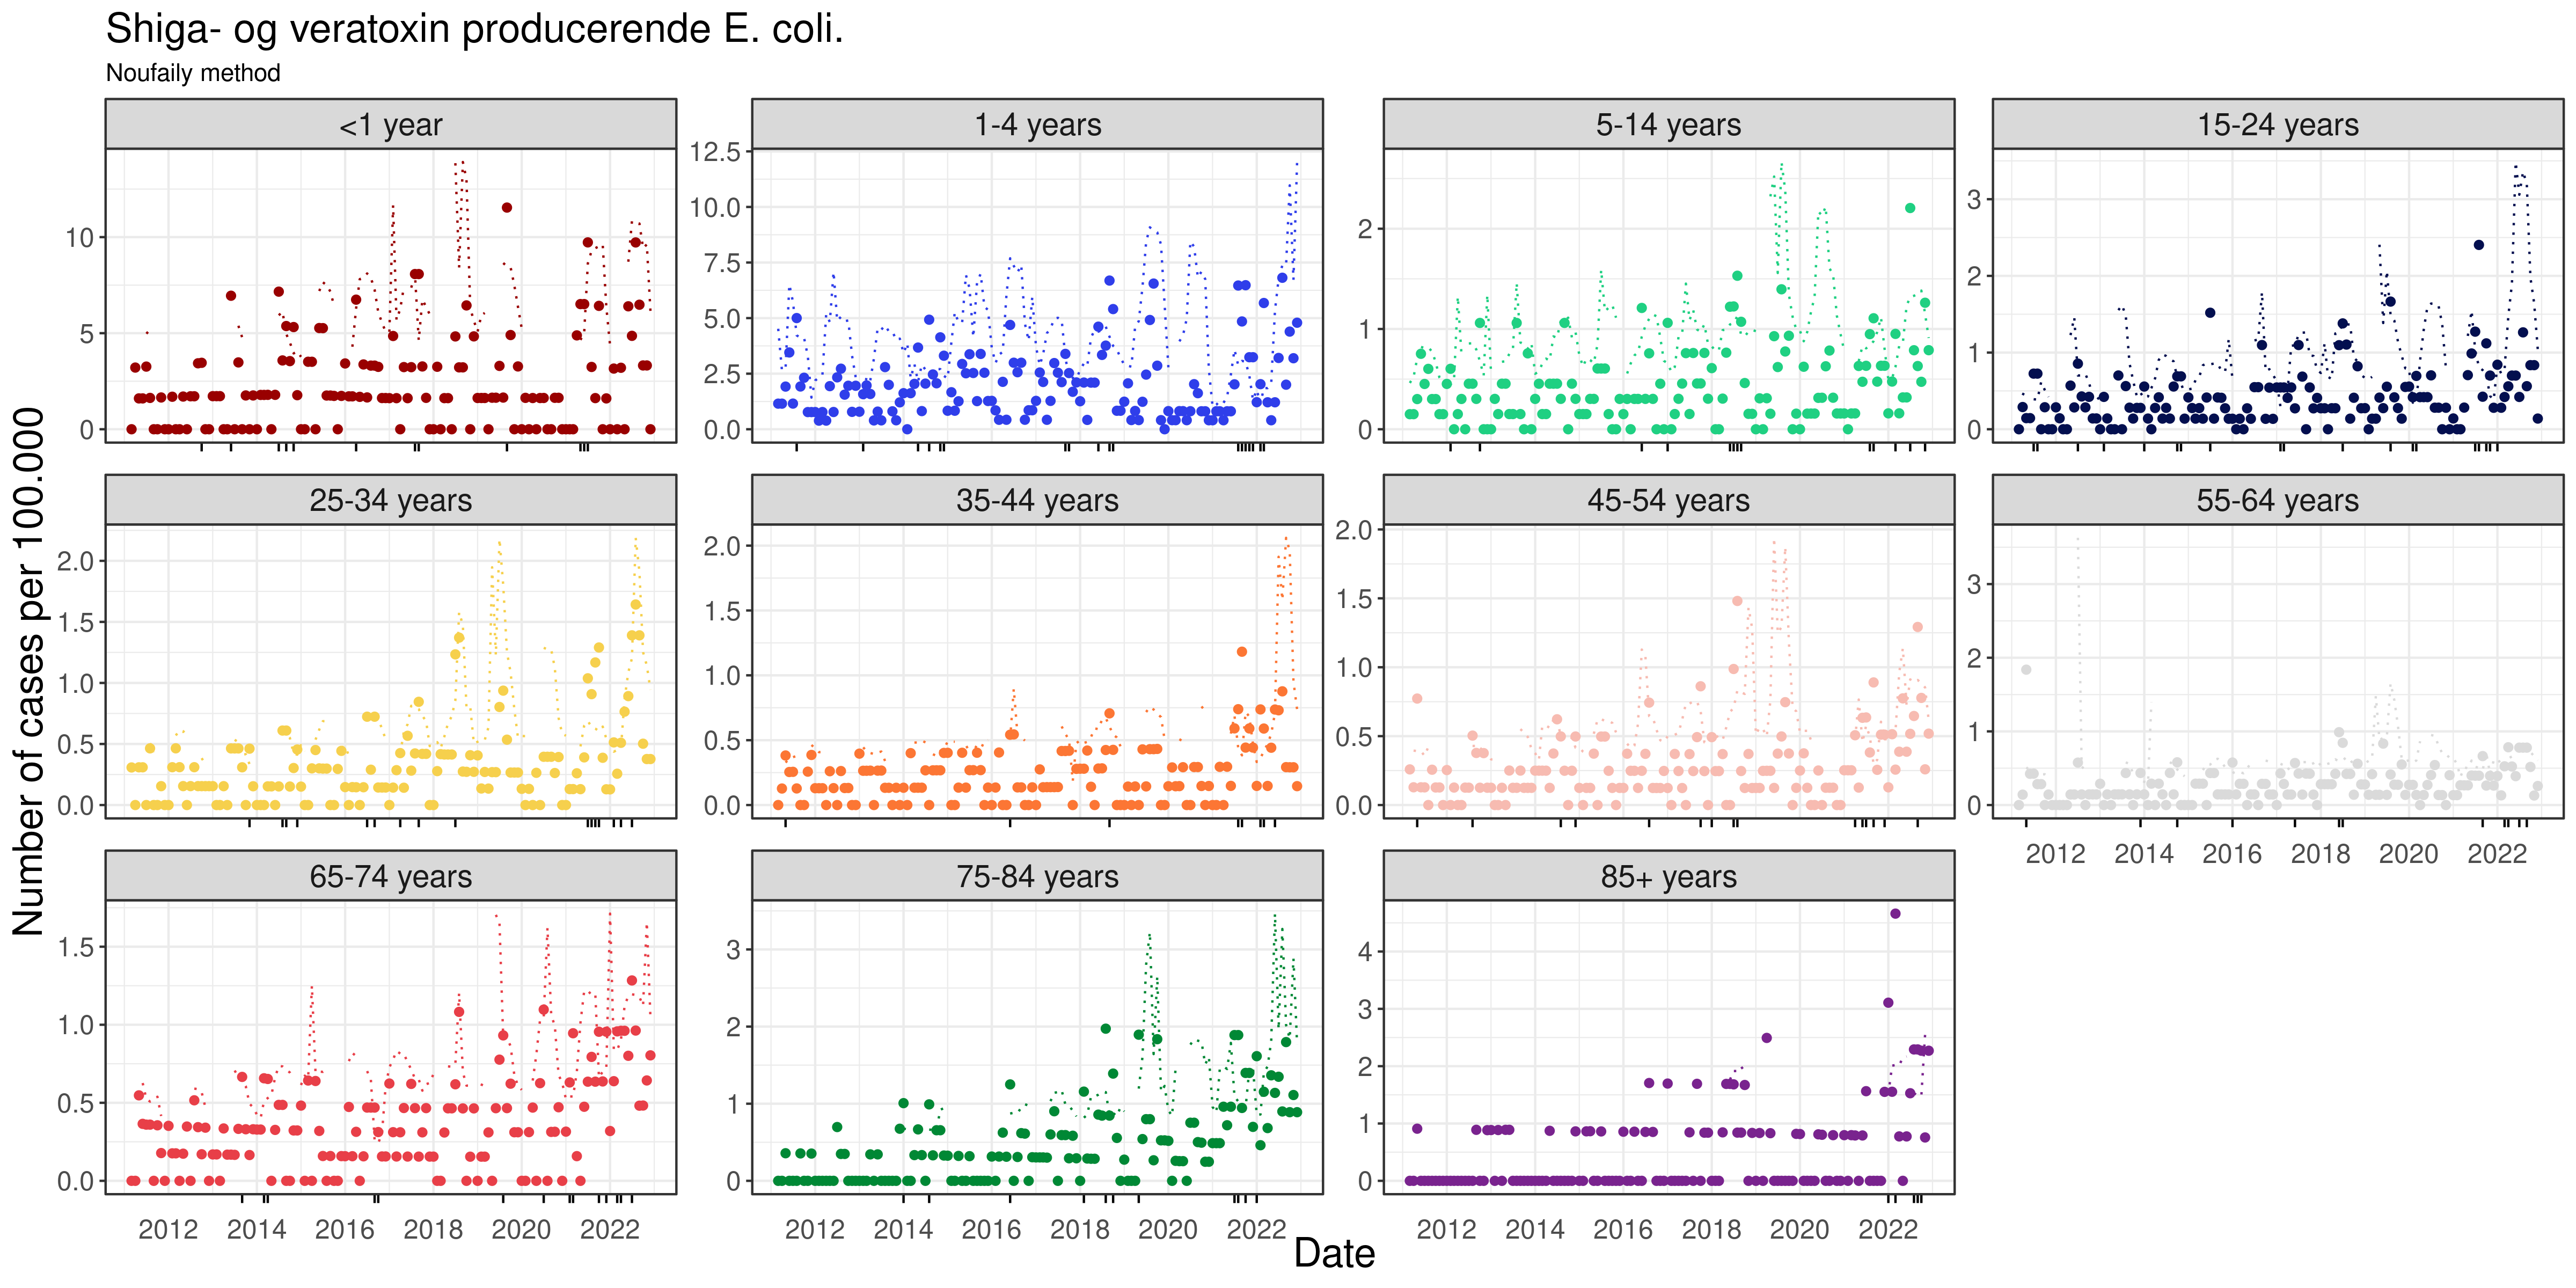
\includegraphics[width=1\linewidth]{../figures/STEC_noufaily}

\normalsize
\end{frame}


\end{document}
